% !TEX root = document.tex

\chapter{\label{chap:cpscomp}Compiling with Continuations}

In this chapter we will develop the first version of the LamToWat compiler that translates the \icode{Lam} language into the \icode{Wat} language. Our compiler will be written in Haskell \autocite{haskellhomepage} and as such \icode{Lam} and \icode{Wat} are implemented as Haskell data types. We follow a minimal version of the approach by \citeauthor{DBLP:books/daglib/0022396} \autocite{DBLP:books/daglib/0022396}. Consequently, the CPS language will serve as IR and have its own data type \icode{Cps}. The purpose of building LamToWat is to examine and then improve its IR. The complexity of CPS conversion and difficulties with the untyped IR transformations will become apparent. If we can improve upon the already favorable features of CPS, we are creating a better IR to program in. Although we are not concerned with the peripherals of the compiler, an IR is not used in a vacuum. We want to examine the compiler passes that map to and from the IR as well as the ones that map to the IR itself. Additionally, to test the compiler we will need to read lambda calculus source files.

What makes CPS favorable as an IR is that it makes control flow and data flow explicit. These features nicely represent the objective of a compiler: translating from a high-level to a low-level language by describing abstractions in finer detail. CPS uses special functions, called 'continuations', to describe more complex control flow constructs. The fact that continuations are special functions becomes essential when translating languages with first-class functions.

LamToWat is a multipass compiler. This means that multiple passes over the IR will be made, each transforming a part of the representation. The complete compiler comprises these IR transformations with additional passes to read in source files and emit \icode{Wat} (the output). Each compiler pass wil have a type that looks like: \icode{pass :: from -> effect to}. \icode{from} and \icode{to} indicate the types of the data structures that are translated. The \icode{effect} type describes all the effects of the transformation in which the \icode{to} type is wrapped. For example our \icode{Lam} parser will have the type \icode{s2l :: String -> Parser Lam}. To continue with the next pass we need to 'extract' our data type by handling its effects. This is done with special functions called handlers. We compose the orginal function together with its handlers to get the complete compiler pass, which will have a simpler type \icode{str2lam :: String -> Lam}.

The data types we will be using are \icode{Lam}, \icode{Cps}, and \icode{Wat}. To read in source files we also need the data type \icode{String}. The monads/effects we will be using are created by combining the standard monad transformers from Haskell's monad transformer library package \icode{mtl} and the \icode{Parser} monad of the \icode{parsec} package. Handlers for these effects are included in their respective packages. LamToWat will be made up of the following sequences of transformations, see figure \ref{fig:lam2watv1org}.

\begin{figure}
\begin{gather*}
  String \xto{str2lam} Lam \xto{lam2cps} Cps \xto{cps2cps} Cps \xto{cps2wat} Wat \xto{show} String
\end{gather*}
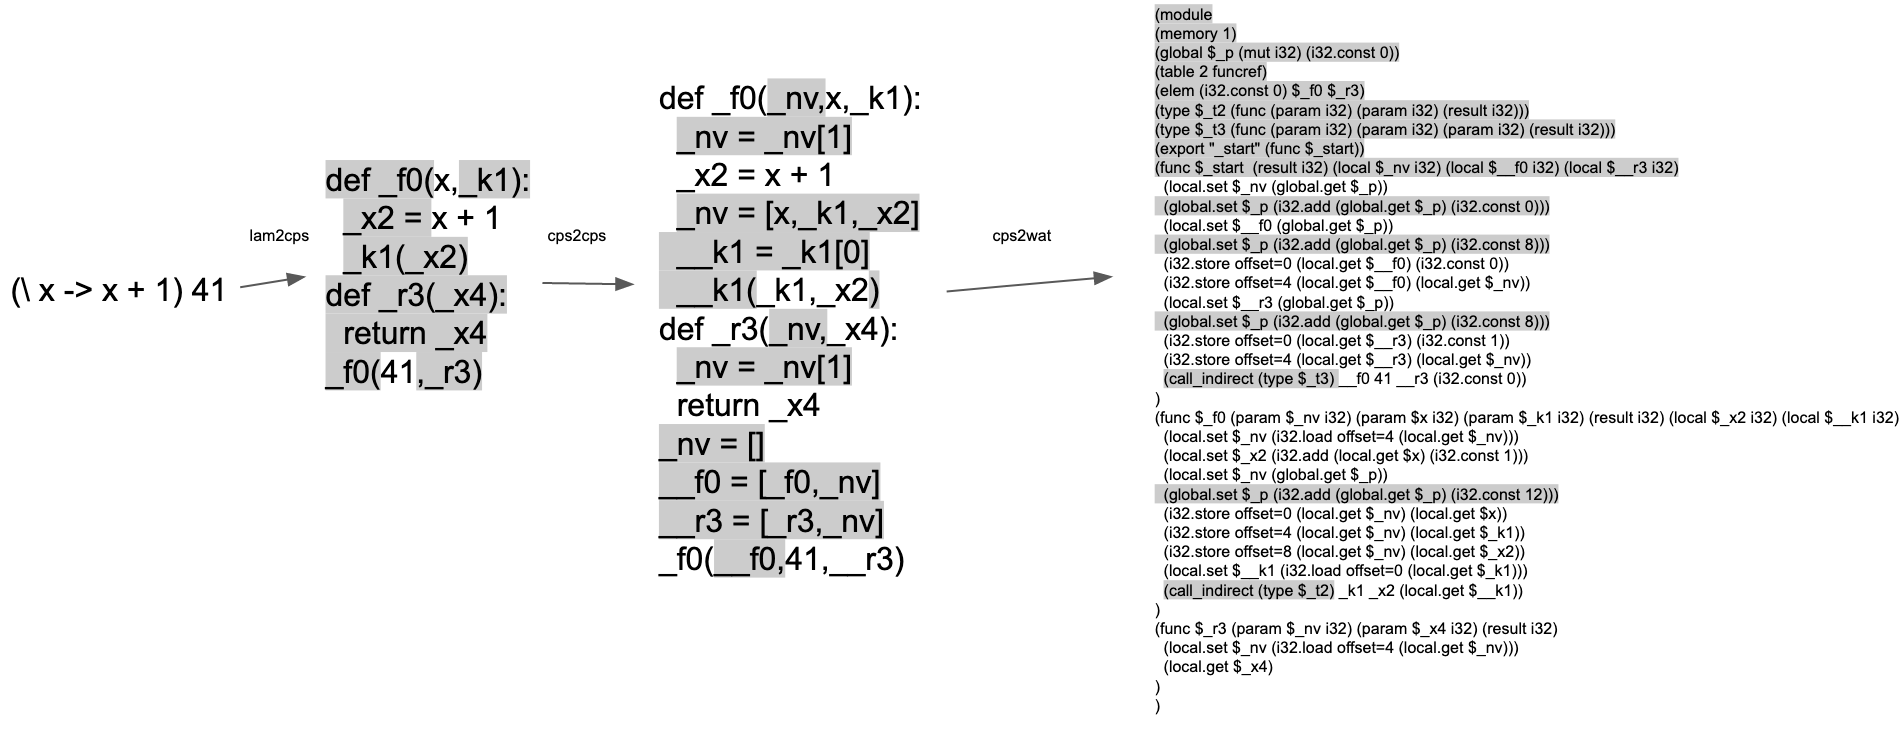
\includegraphics[width=1\textwidth]{./img/cps.png}
\caption{LamToWat Version 1: compiler organization. New pieces of code are highlighted in grey.}
\label{fig:lam2watv1org}
\end{figure}

LamToWat is split into a front-end and a back-end. The front-end of the compiler is made up of parsing \icode{str2lam}, and CPS conversion \icode{lam2cps}. We will not discuss  parsing in detail, as it is irrelevant to the research in this thesis. We will focus on the transformation that involve the IR. We use \icode{megaparsec} to build a parser for our compiler. The back-end of LamToWat consist of three transformations on the IR: closure conversion, hoisting, and emitting \icode{cps2wat}. In the first version of the compiler hoisting and closure conversion are combined in \icode{cps2cps}.

LamToWat is validated by checking that after each transformation the same result is obtained by interpreting that data type with our own interpreter. We match the output of the interpreted \icode{Lam}, \icode{Cps}, and \icode{Wat}. We will use the same set of lambda calculus programs to test both versions of LamToWat. We provide call-by-value semantics for the \icode{Lam} language to be able to compare it to the semantics of \icode{Cps} and \icode{Wat}. The domains of \icode{Lam}, \icode{Cps}, and \icode{Wat} differ making it harder to determine if programs have the same semantics. Moreover, it is not possible to compare functions. To circumvent this problem we will only compare programs that will have integer results.

The following sections will first describe the data types \icode{Lam}, \icode{Cps}, and \icode{Wat} used in LamToWat with specific attention to \icode{Cps}. Then we will adhere to the organization of the compiler and discuss the relevant compiler passes over these data types in the order described in figure \ref{fig:lam2watv1org}.

\section{\label{section:datatypes}Data Types}
The data types of LamToWat will be implemented as Haskell data types. Haskell data types are indicated with the \icode{data} keyword. Every data type has a name, which comes after the keyword. Then a number of constructors follow separated by vertical bars. Data types can be recursively defined. Type aliases indicated with the \icode{type} keyword are also used; providing new names for existing data types.

\subsection{\label{subsection:expdata}The Lam Language}
The \icode{Lam} data type represents the abstract syntax tree of the lambda calculus. The three constructors for \icode{Lam}bda abstraction, \icode{App}lication, and \icode{Var}iables encompass the standard definition of the lambda calculus. Two constructors for \icode{Num}bers and \icode{Add}ition are added to make basic arithmetic possible. The lambda calculus is one of the smallest functional languages that still has many of the interesting properties of functional languages, such as first-class functions and recursion. Moreover, the lambda calculus is well-studied \autocite{barendregt1984lambda}. Programs written in the lambda calculus will be used for testing LamToWat.

% moet in figure?
\begin{lstlisting}[language=Haskell]
data Lam
  = Lam String Lam
  | App Lam Lam
  | Add Lam Lam
  | Var String
  | Num Int
\end{lstlisting}

Two programs will be used as running examples throughout this thesis to show how the compilation process works. In the lambda calculus they are written as follows.

\begin{lstlisting}[language=Haskell]
(\ x -> x + 1) 41
(\ x -> (\ y -> x + y)) 13 29
\end{lstlisting}

We use the same notation as Haskell uses for the lambda calculus, \icode{\} and \icode{->} are used for lambda abstraction and a space is used for application. Both programs are valid inputs to LamToWat and contain all five of the lambda calculus constructs. The first program \icode{(\ x -> x + 1) 41} applies an anonymous function that adds 1 to its argument \icode{x} to the number 41. The second programs \icode{(\ x -> (\ y -> x + y)) 13 29} applies a nested anonymous function that adds its arguments to the numbers 13 and 29. We choose a program with nested functions and a program without nested functions as examples to display the compilation of this language feature separately. Translated to the \icode{Lam} language the programs are written as follows.

\begin{lstlisting}[language=Haskell]
App (Lam "x" (Add (Var "x") (Num 1))) (Num 41)
App (App (Lam "x" (Lam "y" (Add (Var "x") (Var "y")))) (Num 13)) (Num 29)
\end{lstlisting}

You can instantly see why we prefer the shorter notation. \icode{Lam} expressions contain lots of brackets and constructor names. These declare the order of operations and the sort of (sub)-expression we are dealing with. This information is required by the compiler. Our parser program converts from the first notation to the \icode{Lam} language.

Both example programs evaluate to the number 42 by substituting the arguments into the functions. The semantics of these two programs is given by an interpreter function called \icode{lam2dom}, which maps \icode{Lam} expression to a \icode{Dom}ain data type. We use a reader monad to keep track of bound variables. We choose call-by-value semantics, which means that arguments to functions are evaluated before the function is applied to them. For our example programs this does not matter, because in both cases the arguments are simple integers. It becomes relevant when we want to express more complicated functions in the lambda calculus, like a fixpoint.

\subsection{\label{subsection:cpsdata}The Cps Language}
We follow the CPS language data type definition and semantics by \citeauthor{DBLP:books/daglib/0022396} \autocite{DBLP:books/daglib/0022396} with some minor adjustments. It is used as IR because it facilitates compiler transformations relevant to functional programming languages. The data type is similar to the control flow graph of a program. Control flow is modeled with functions and function calls. Data flow is modeled with records. LamToWat uses CPS to transform nested, higher-order functions to simple functions. The semantic \icode{Dom}ain data type of \icode{Cps} consists of functions, integer numbers, and records.

\icode{Cps} functions are made up of a name, argument names, and a body. They are defined in mutually recursive \icode{FIX}ed function blocks. Values are either \icode{INT}egers, \icode{VAR}iables, or \icode{LABEL}s. \icode{LABEL}s are used for proper function names appearring in \icode{FIX}es, \icode{VAR}iables for everything else including continuations. The CPS language enforces the distinction between \icode{Val}ues and \icode{Cps} expressions by putting them in separate data types. All expressions except \icode{APP} and \icode{DONE} have a \icode{Cps} continuation as their last argument. Since the \icode{ADD}, \icode{RECORD}, and \icode{SELECT} expressions produce a value, they name it before continuing with their \icode{String} argument. \icode{DONE} helps us to define the function that translates a source language into CPS. As this expression represents a return statement, it does not adhere to continuation-passing style. No problems are caused by it, because we will make sure that it is the final expression of our programs. This makes it a global return of the program itself, not of a function.

Variable names in \icode{Cps} are represented by simple strings. This is a design choice as it allows for nonsense programs that use undefined variables, but also for easy manipulation of variables and generation of variable names.

\begin{lstlisting}[language=Haskell]
data Val
  = INT Int
  | VAR String
  | LABEL String
  
type Fun = (String, [String], Cps)
data Cps
  = APP Val [Val]
  | DONE Val
  | RECORD [Val] String Cps
  | SELECT Int Val String Cps
  | ADD Val Val String Cps
  | FIX [Fun] Cps
\end{lstlisting}

The \icode{Cps} data type guarantees that compiler transformations can be easily implemented by enforcing the following properties. CPS also requires all user functions to have an extra continuation argument. This requirement is not enforced by the data type, but needs to be fulfilled in order for it to be proper CPS.

\begin{itemize}
\item Functions do not return, instead the last thing a function does is call a continuation.
\item Function parameters can only be values.
\item All intermediate values have names.
\end{itemize}

To illustrate how the \icode{Cps} data type is used we will translate the lambda calculus example \icode{(\ x -> x + 1) 41} to \icode{Cps}. We define a function in a \icode{FIX} block with name \icode{f} and argument \icode{x}. The body of this function adds \icode{x} and 1, names the result \icode{r}, and returns this result. Finally, we apply \icode{f} to 42.

\begin{lstlisting}[language=Haskell]
  FIX [("f", ["x"], ADD (VAR "x") (INT 1) "r" (DONE "r"))] (APP (VAR "f") [INT 41])
\end{lstlisting}

\icode{Cps} expressions can become large and unwieldy, especially in later stages of LamToWat. For this reason we use a simpler Python-like notation to describe \icode{Cps}. LamToWat can print \icode{Cps} with the same notation. In this notation the translated example is written as follows.

\begin{lstlisting}[language=Haskell]
def f(x):
  r = x + 1
  return r
f(41)
\end{lstlisting}

\icode{FIX} blocks have been replaced by indented \icode{def}s. The assignment of intermediate variables is indicated with a \icode{=}. Function application is performed by placing braces around the arguments and commas in between arguments. Records will be created with square brackets \icode{[1,2,3]} and selecting from records will be done with square brackets too \icode{r[0]}. The \icode{DONE} constructor is represented by the \icode{return} keyword. Variables generated by the compiler will be prefixed with a '\icode{_}'.

\subsection{\label{subsection:webdata}The Wat Language}
The \icode{Wat} language is a hierarchical, high-level assembly language and a simplification of WebAssembly \autocite{webassemblyhomepage}. As the final language in the compilation process it gives some guarantees about the well-formedness of the output of the compiler. The fundamental unit of code is a \icode{Module} made up of a list of functions with bodies made up of \icode{Exp}.

We have chosen \icode{Wat} as the output language of LamToWat, because it is a relatively high-level language without first-class functions. It can be easily translated to WebAssembly, but still has enough abstraction to be able to target other languages. The absence of first-class functions requires LamToWat to actually compile the \icode{Lam} language, which does have this feature. By keeping the output of LamToWat as a Haskell data type, we can compare the semantics of the \icode{Lam}, \icode{Cps}, and \icode{Wat} data types more easily.

We see that \icode{Wat} is quite similar to \icode{Cps}, this makes it easy to translate from \icode{Cps} to \icode{Wat} after closure conversion and hosting. The \icode{RECORD} and \icode{SELECT} constructors are replaced with \icode{Malloc}, \icode{Store}, and \icode{Load}. The \icode{LABEL} constructor from \icode{Val} is not used, because functions are now represented by integers serving as an index into the module's function list. \icode{FIX} is replaced with a top-level \icode{Module}, ensuring that there are no nested functions anymore.

The \icode{Dom}ain of \icode{Wat} consists of integers serving as numbers, function pointers, and heap pointers. Instead of creating record values, our three heap operators will manipulate a piece of memory of constant size. This means that just like in real WebAssembly we can access out of bounds memory and crash our program.

\begin{lstlisting}[language=Haskell]
data Wat = Module [(String,[String],Exp)] Exp

data Exp
  = Malloc Int String Exp
  | Store Int Val Val Exp
  | Load Int Val String Exp
  | Add Val Val String Exp
  | App Val [Val]
  | Done Val
\end{lstlisting}

Let's see how our example program looks in the \icode{Wat} language. The only real difference with \icode{Cps} is the use of the an \icode{INT} instead of a \icode{LABEL} to indicate a function pointer.

\begin{lstlisting}[language=Haskell]
Module 
  [("f",["x"],Add (VAR "x") (INT 1) "r" (Done (VAR "r")))]
  (App (INT 0) [INT 41])
\end{lstlisting}

We can print \icode{Wat} as 'real' WebAssembly that can be compiled and ran by WABT \autocite{wabt}. When we translate to WebAssembly our program becomes a lot longer and there are many new keywords. WebAssembly requires the programmer to declare some extra information, which leads to a lot of syntactic noise. This information can be deduced from the previous simpler \icode{Wat} expression, so we can generate the syntax automatically. The first seven lines of the printed WebAssembly program declare that there is one page of mutable global memory and a mutable heap pointer. We declare one function reference of the function \icode{f}. This function has type \icode{_t1}. In order to run the program we need to export the \icode{_start} function. Following the preamble we see the entry point of our program in the form of the function \icode{_start} and our original function \icode{f}. Function signatures now include a result type (which is always \icode{i32}) and all locally used variables indicated with the \icode{local} keyword. When we call a function we indicate the type of that function with the \icode{type} keyword.

\begin{lstlisting}
(module
(memory 1)
(global $_p (mut i32) (i32.const 0))
(table 1 funcref)
(elem (i32.const 0) $f)
(type $_t1 (func (param i32) (result i32)))
(export "_start" (func $_start))
(func $_start  (result i32) 
  (call_indirect (type $_t1) (i32.const 41) (i32.const 0))
)
(func $f (param $x i32) (result i32) (local $r i32)
  (local.set $r (i32.add (local.get $x) (i32.const 1)))
  (local.get $r)
)
)
\end{lstlisting}

\section{\label{section:transforms}Transformations}
Transformations or compiler passes of LamToWat will be implemented as Haskell functions. These functions will transform the data types of the previous section. A transformation can convert a data type to a different data type, or to the same data type with certain properties. The (side-)effects of the transformations are modeled using monads \autocite{DBLP:conf/lics/Moggi89}. Monads allow us to write effectful code in a pure functional language like Haskell. We can combine monadic effects by using monad transformers \autocite{DBLP:conf/popl/LiangHJ95}. We have the convention that for every transformation we name this combined monad for effects \icode{M}.

\subsection{\label{subsection:cpsconvert}CPS Conversion}
CPS conversion will transform the \icode{Lam} data type into the \icode{Cps} data type. By converting our program to continuation-passing style we make control flow and data flow explicit. In practice this means that we generate fresh variable names for intermediate values and use a continuation that indicates the order of expressions.

\citeauthor{DBLP:books/daglib/0022396} describes a CPS conversion function that takes an extra metacontinuation as argument. It also assumes some way of generating fresh variable names, which is not further specified. In haskell the signature of such a fuction would look as follows. It uses a state monad for fresh variable name generation.

\begin{lstlisting}[language=Haskell]
Lam -> (Val -> State Int Cps) -> State Int Cps
\end{lstlisting}

Our CPS conversion function uses the continuation monad to provide the continuation. Fresh variables are still generated using the state monad. We use Haskell's \icode{do}-notation to write our monadic conversion function in an imperative style. Our monad \icode{M} will have the following type.

\begin{lstlisting}[language=Haskell]
type M = ContT Cps (State Int)
\end{lstlisting}

\icode{l2c} is split up into cases for each constructor of \icode{Lam}. The values \icode{Var} and \icode{Num} are converted to CPS values. To convert the anonymous function \icode{Lam} we generate fresh variables \icode{f} and \icode{k} to name the function and its continuation. We pass the function name to the metacontinuation \icode{c}. We convert the body of the function \icode{e}, giving it a metacontinuation which calls the continuation with the result \icode{z}. Finally, we construct a \icode{FIX} to contain our converted function and update continuation \icode{c'}. The \icode{App} and \icode{Add} cases follow a similar approach.

\begin{lstlisting}[language=Haskell]
l2c :: Lam -> M Val
l2c (Var x) = return (VAR x)
l2c (Num i) = return (INT i)
l2c (Lam x e) = ContT (\ c -> do
  f <- fresh "f"
  k <- fresh "k"
  cf <- runContT (l2c e) (\ z ->
          return (APP (VAR k) [z]))
  c' <- c (LABEL f)
  return (FIX [(f,[x,k],cf)] c'))
l2c (App e1 e2) = do
  v1 <- l2c e1
  v2 <- l2c e2
  ContT (\ c -> do
    r <- fresh "r"
    x <- fresh "x"
    c' <- c (VAR x)
    return (FIX [(r,[x],c')] (APP v1 [v2, LABEL r])))
l2c (Add e1 e2) = do
  v1 <- l2c e1
  v2 <- l2c e2
  ContT (\ c -> do
    x <- fresh "x"
    c' <- c (VAR x)
    return (ADD v1 v2 x c'))
\end{lstlisting}

How the \icode{l2c} function works is not obvious. We have to generate variable names, pass these to the continuation and sometimes wrap the resulting values in a \icode{FIX}. This is quite complex, control flow should be easier to describe. For binary operators like \icode{App} and \icode{Add} we want to evaluate the left argument first (arbitrarily chosen order), the right argument second and finally add the two resulting values. We would like to write something like the following instead of generating a variable name and exposing the metacontinuation using a monad.

\begin{lstlisting}[language=Haskell]
l2c' (Add e1 e2) = do
  v1 <- l2c' e1
  v2 <- l2c' e2
  add v1 v2
\end{lstlisting}

The case for \icode{App} is especially complicated as we have to create a return point function to serve as continuation argument to the final application. Keeping track of continuations becomes even more non-trivial when we have multiple of them. For example when we want to have exception handlers in our source language.

We give an example of CPS converting our example \icode{(\ x -> x + 1) 41} with \icode{lam2cps} to see how it works. \icode{lam2cps} is a composition of \icode{l2c} and the handlers of the state and continuation monad, which gives it type \icode{Lam -> Cps}, where \icode{l2c} has type \icode{Lam -> M Val}, with the \icode{Cps} expression hidden in the continuation monad part of \icode{M}. \icode{lam2cps} takes a simple \icode{Lam} expression and prints out \icode{Cps}. Variables generated by the \icode{l2c} are prefixed with a \icode{_}.

\begin{lstlisting}[language=Haskell]
def _f0(x,_k1):
  _x2 = x + 1
  _k1(_x2)
def _r3(_x4):
  return _x4
_f0(41,_r3)
\end{lstlisting}

We see two functions \icode{_f0} and \icode{_r3} have been created. The first represents our original function with an additional continuation argument \icode{_k1}. The body of the function adds the number one to \icode{x} and passes the result to the continuation. The other function represents a return point. In this case the return point of the entire program as it uses the \icode{DONE} constructor. Finally, we see the call to \icode{_f0} where we pass the original argument and the return function as the continuation.

\subsection{\label{section:closconvert}Closure Conversion}
Closure conversion transforms the \icode{Cps} data type into the \icode{Cps} data type where functions do not contain free variables. The free variables of a function are passed to the function via an extra argument. We will package a function with its free variables, this package is called a 'closure'. \icode{Cps} implements closures as records, where the first argument is a function pointer (implemented as a \icode{LABEL}) and the following elements are free variables. We use a reader monad to keep track of variables in scope and a writer monad to collect function at the top-level.

There are many approaches to generating closures. We take an approach optimized for simplicity. When we encounter a \icode{FIX} we ask what variables are in scope. For each function we add an extra first argument \icode{_nv}: the closure record. We prefix the function body with selecting and naming all variables in scope from the closure record. When we encounter an \icode{APP} we create a record with all variables in scope and pack it with the function pointers that are in function or argument position off the \icode{APP} to create a closure and rename it by prefixing an underscore. To apply the closure we select the first argument from the respective record and apply it to itself and its original arguments. For the other constructors we simply update the environment with their assigned names.

We now use a different monad \icode{M} to keep track of the environment and collect our functions. \icode{M} consists of a combination of the Writer and the Reader monad. The first one is used for collecting functions and the second one to keep track of the environment. \icode{M} has the following type. The order of transformers is arbitrary.

\begin{lstlisting}[language=Haskell]
type M =  WriterT [Fun] (Reader [String])
\end{lstlisting}

Care must be taken to ensure that the closest variable binds (lexical scope). This means that when we enter a function we bring into scope the environment variables that are not arguments of the function, see the helper function \icode{open}.

\begin{lstlisting}[language=Haskell]
c2c :: Cps -> M Cps
c2c (FIX fs e) = do
  nv <- ask
  fs' <- mapM (\ (f,as,b) -> do
        b' <- local (++ as) (c2c b)
        return (f,_nv:as,open b' as nv)) fs
  tell fs'
  c2c e
c2c (APP v vs) = do
  nv <- ask
  let vs' = rename vs
  let app = apply v vs'
  return (close app (v:vs) nv)
c2c (DONE v) = return (DONE v)
c2c (RECORD vs x e)  = do
  e' <- local (++ [x]) (c2c e)
  return (RECORD vs x e')
c2c (SELECT i v x e) = do
  e' <- local (++ [x]) (c2c e)
  return (SELECT i v x e')
c2c (ADD v1 v2 x e)  = do
  e' <- local (++ [x]) (c2c e)
  return (ADD v1 v2 x e')

open :: Cps -> [String] -> [String] -> Cps
open e as nv = SELECT 1 (VAR _nv) _nv
  (foldr (\ (i,x) b -> if x `elem` as then b else SELECT i (VAR _nv) x b) e (zip [0..] nv))

apply :: Val -> [Val] -> Cps
apply (LABEL f) vs = APP (LABEL f) (VAR (_p f) : vs)
apply (VAR f) vs = SELECT 0 (VAR f) (_p f) (APP (VAR (_p f)) (VAR f : vs))

close :: Cps -> [Val] -> [String] -> Cps
close e vs nv = RECORD (map VAR nv) _nv
  (foldr (\ v b -> case v of LABEL f -> RECORD [v,VAR _nv] (_p f) b; _ -> b) e vs)

rename :: [Val] -> [Val]
rename vs = map (\ v -> case v of LABEL f -> VAR (_p f); _ -> v) vs

_p = ('_' :)
_nv = "_nv"
\end{lstlisting}

The main defect of \icode{c2c} is that it gives no indication of the fact that our \icode{Cps} expressions no longer contain \icode{FIX} expressions. When we encounter a \icode{FIX}, we use the \icode{tell} function to write all functions to a list. It is obvious from the implementation that they are no longer present, however, the type of the transformation gives no recognition of this fact. If we were to pass a \icode{Cps} expression to the next pass of the compiler that has nested \icode{FIX}es, it would cause an error.

We will again look at an example to see how this function works. We closure convert \icode{(\ x y -> x + y) 13 29} using the \icode{cps2cps} function, which is a composition of \icode{c2c} and monad handlers.

\begin{lstlisting}[language=Haskell]
def _f2(_nv,y,_k3):
  _nv = _nv[1]
  x = _nv[0]
  _k1 = _nv[1]
  _x4 = x + y
  _nv = [x,_k1,y,_k3,_x4]
  __k3 = _k3[0]
  __k3(_k3,_x4)
def _f0(_nv,x,_k1):
  _nv = _nv[1]
  _nv = [x,_k1]
  __f2 = [_f2,_nv]
  __k1 = _k1[0]
  __k1(_k1,__f2)
def _r7(_nv,_x8):
  _nv = _nv[1]
  _x6 = _nv[0]
  return _x8
def _r5(_nv,_x6):
  _nv = _nv[1]
  _nv = [_x6]
  __r7 = [_r7,_nv]
  __x6 = _x6[0]
  __x6(_x6,29,__r7)
_nv = []
__f0 = [_f0,_nv]
__r5 = [_r5,_nv]
_f0(__f0,13,__r5)
\end{lstlisting}

The first thing we notice is that functions are no longer nested. We also see the addition of records and selection. We have four functions representing our original two functions and the two applications. We can see how the original function bodies are prefixed with opening closures and postfixed with creating closures before application. All functions have an extra \icode{_nv} argument. If a function was originally nested more deeply, it will open and create a closure with more elements, because there will be more variables in scope. This is the case for the function \icode{_f2}, where the actual addition of \icode{x} and \icode{y} happens. The first closure that is created in our program before calling \icode{_f0} is empty. This is because at the top level there are no free variables. The two closures for \icode{_f0} and \icode{_r5} named \icode{__f0} and \icode{__r5}, respectively, are a sort of dummy closure only containing a function pointer and a empty environment.

\subsection{\label{section:emit}Emitting}
Emitting transforms the \icode{Cps} data type into the \icode{Wat} data type. We first create a list of function names \icode{ns}. This way we can map function names to indices. The most interesting parts of the transformation are for the \icode{RECORD} case and \icode{LABEL} case. \icode{RECORD}s are transformed into a combination of \icode{Malloc} and \icode{Store}, because \icode{Wat} does not support such a high level abstraction, but just has a heap. \icode{LABEL}s are mapped to their index in the list of function names. If the name is not present, the function will fail with an error.

This transformation could benefit from the reuse of constructors. We see that \icode{APP} is transformed to its \icode{Wat} counterpart \icode{App}. We could just leave these parts of the data type untouched and only show the essence of the transformation, it would benefit both the reader and the writer of this code. What the transformation does would be more explicit and less code naturally leads to a smaller number of errors.

\begin{lstlisting}[language=Haskell]
cps2wat :: Cps -> Wat
cps2wat (FIX fs e) = Module fs' (go e)
  where ns :: [String]
        ns = map (\ (f,as,b) -> f) fs

        fs' :: [(String,[String],Exp)]
        fs' = map (\ (f,as,b) -> (f,as,go b)) fs

        go :: Cps -> Exp
        go (APP v vs) = App (vo v) (map vo vs)
        go (DONE v) = Done (vo v)
        go (RECORD vs x e) = Malloc (length vs) x
          (foldr (\ (i,v) -> Store i (VAR x) (vo v)) (go e) (zip [0..] vs))
        go (SELECT i v x e) = Load i (vo v) x (go e)
        go (ADD v1 v2 x e) = Add (vo v1) (vo v2) x (go e)

        vo v = case v of
          LABEL x -> INT (fromJust (x `elemIndex` ns))
          _       -> v
\end{lstlisting}

Let's look at a final example for the function \icode{(\ x -> x + 1) 41}. We have no side-effects as can be seen in the signature for \icode{cps2wat}, so we will simply use this function.

\begin{lstlisting}[language=Haskell]
(module
(memory 1)
(global $_p (mut i32) (i32.const 0))
(table 2 funcref)
(elem (i32.const 0) $_f0 $_r3)
(type $_t2 (func (param i32) (param i32) (result i32)))
(type $_t3 (func (param i32) (param i32) (param i32) (result i32)))
(export "_start" (func $_start))
(func $_start  (result i32) (local $_nv i32) (local $__f0 i32) (local $__r3 i32)
  (local.set $_nv (global.get $_p))
  (global.set $_p (i32.add (global.get $_p) (i32.const 0)))
  (local.set $__f0 (global.get $_p))
  (global.set $_p (i32.add (global.get $_p) (i32.const 8)))
  (i32.store offset=0 (local.get $__f0) (i32.const 0))
  (i32.store offset=4 (local.get $__f0) (local.get $_nv))
  (local.set $__r3 (global.get $_p))
  (global.set $_p (i32.add (global.get $_p) (i32.const 8)))
  (i32.store offset=0 (local.get $__r3) (i32.const 1))
  (i32.store offset=4 (local.get $__r3) (local.get $_nv))
  (call_indirect (type $_t3) (local.get $__f0) (i32.const 41) (local.get $__r3) (i32.const 0))
)
(func $_f0
 (param $_nv i32) (param $x i32) (param $_k1 i32) (result i32) (local $_x2 i32) (local $__k1 i32)
  (local.set $_nv (i32.load offset=4 (local.get $_nv)))
  (local.set $_x2 (i32.add (local.get $x) (i32.const 1)))
  (local.set $_nv (global.get $_p))
  (global.set $_p (i32.add (global.get $_p) (i32.const 12)))
  (i32.store offset=0 (local.get $_nv) (local.get $x))
  (i32.store offset=4 (local.get $_nv) (local.get $_k1))
  (i32.store offset=8 (local.get $_nv) (local.get $_x2))
  (local.set $__k1 (i32.load offset=0 (local.get $_k1)))
  (call_indirect (type $_t2) (local.get $_k1) (local.get $_x2) (local.get $__k1))
)
(func $_r3 (param $_nv i32) (param $_x4 i32) (result i32) 
  (local.set $_nv (i32.load offset=4 (local.get $_nv)))
  (local.get $_x4)
)
)
\end{lstlisting}

We see that our program has become quite large. Moreover, we notice that \icode{i32.load} and \icode{i32.store} are used instead of records. Local variables are prefixed with a dollar sign \icode{$} and are updated and accessed using \icode{local.set} and \icode{local.get}. Functioons now have have signatures with types that specify their \icode{param}eters, \icode{result}, and \icode{local} variables. Function pointers are implemented as integers instead of \icode{LABEL}s. For example: the first function call on the last line of the body of the \icode{_start} function is to an integer constant \icode{0}, instead of the original function name \icode{_f0}. 

\section{\label{section:summarycps}Chapter Summary}
In this chapter we have shown how to build a compiler that translates \icode{Lam} into \icode{Wat}. We used three data types: \icode{Lam}, \icode{Cps}, and \icode{Wat}. By applying the transformations \icode{str2lam}, \icode{lam2cps}, \icode{cps2cps}, and \icode{cps2wat} to a well formatted lambda calculus string, we obtain a low-level language output that can be printed as WebAssembly. To examine the transformations we provide pretty-printed output to more easily show the difference between compiler passes. By looking at two example lambda expressions we tracked the state of our program throughout its compilation.

We identified problems with the transformations on the data types and the data types itself. These are summarized as follows:

\begin{itemize}
\item Complex specification of control flow in \icode{l2c}\\\\
\icode{l2c} is itself written in CPS. We used the continuation monad to try and hide this fact, however the function requires us to expose the metacontinuation. This leads to a confusing specification of control flow where the programmer needs to constantly switch between continuation and metacontinuation.
\item No types to indicate change of \icode{Cps} after \icode{c2c}\\\\
Closure conversion has type \icode{c2c :: Cps -> WriterT [Fun] (Reader [String]) Cps}. If we ignore the monadic effects for a moment we obtain the simpler type \icode{([Fun],Cps)}. The \icode{Cps} data type is free to contain \icode{FIX} expressions. We want to guarantee that it does not and that functions are thus no longer nested. All function definitions should be contained in the function list and their bodies should be made up of expression containing only addition, records, and application.
\item Duplicate constructors in \icode{Cps} and \icode{Wat}\\\\
If we look at both data types we see that addition and application constructors match one-to-one. We would like to only transform \icode{RECORD} expressions into \icode{Malloc} expressions.
\end{itemize}

In the next chapter we will try to alleviate these shortcomings of the first version of our compiler by proposing a new data type: command trees.
